\documentclass[11pt,a4paper]{article}

\usepackage[T1]{fontenc}
\usepackage[utf8]{inputenc}
\usepackage[brazilian]{babel}
\usepackage{lmodern}
\usepackage[margin=2.45cm]{geometry}
\usepackage{microtype}
\usepackage{amsmath}
\usepackage{graphicx}
\usepackage{tikz}
\usepackage{booktabs,tabularx,longtable}
\usepackage{needspace}
\usepackage{xcolor}
\usepackage{listings}
\usepackage{csquotes}
\usepackage[backend=biber,style=numeric,sorting=none,giveninits=true]{biblatex}
\addbibresource{referencias.bib}
\usepackage{hyperref}
\usepackage{xurl}
\usepackage{titlesec}

\definecolor{lameblue}{HTML}{19476B}
\definecolor{codebg}{HTML}{E2E4E7}
\definecolor{codeborder}{HTML}{C4C8CD}
\definecolor{codecomment}{HTML}{27583D}
\definecolor{codestring}{HTML}{783D22}

\definecolor{codefg}{HTML}{20242A}
\definecolor{codekeyword}{HTML}{184B76}

\hypersetup{
  colorlinks=true, linkcolor=lameblue, urlcolor=lameblue, citecolor=lameblue,
  pdftitle={Guia Básico de Python para Ciência de Dados},
  pdfauthor={Phelipe Melo Matos},
  pdfsubject={Guia de Apoio ao minicurso Introdução à Ciência de Dados — EMASC 2026}
}
\urlstyle{same}
\setlength{\emergencystretch}{2em}
\setlength{\parskip}{4pt}
\setcounter{tocdepth}{2}
\titleformat{\section}{\Large\bfseries\color{lameblue}}{\thesection}{0.65em}{}
\titleformat{\subsection}{\large\bfseries\color{lameblue}}{\thesubsection}{0.65em}{}

\lstdefinestyle{guia}{
  basicstyle=\small\ttfamily\color{codefg}, backgroundcolor=\color{codebg},
  frame=single, rulecolor=\color{codeborder}, framesep=6pt,
  keywordstyle=\color{codekeyword}\bfseries,
  commentstyle=\color{codecomment}, stringstyle=\color{codestring},
  columns=fullflexible, keepspaces=true, showstringspaces=false,
  upquote=true, breaklines=true, aboveskip=9pt, belowskip=8pt
}
\lstset{style=guia,language=Python}
\lstnewenvironment{exemplo}[1][]
  {\endgraf\smallskip\noindent\minipage{\linewidth}\lstset{#1}}
  {\endminipage\endgraf\smallskip}
\newcommand{\nota}[2]{\par\smallskip\noindent\textbf{\textcolor{lameblue}{#1.}} #2\par\smallskip}
\newcommand{\codigo}[1]{\texttt{#1}}

\begin{document}

\hypersetup{pageanchor=false}
\begin{titlepage}
  \centering
  \vspace*{1.0cm}
  \begin{tikzpicture}
    \clip (0,0) circle[radius=1.67cm];
    \node[inner sep=0pt] at (0,0)
      {
\includegraphics[width=3.55cm]{figuras/logo-lame.png}};
  \end{tikzpicture}\par
  \vspace{0.8cm}
  {\large Universidade Federal de Sergipe\par}
  {\normalsize Liga Acadêmica Matemática e Empresa\par}
  \vfill
  {\large\bfseries\color{lameblue} Guia de Apoio ao Minicurso\par}
  \vspace{0.6cm}
  {\Huge\bfseries Guia Básico de Python\\[0.14em] para Ciência de Dados\par}
  \vspace{0.6cm}
  {\large Fundamentos de Python, Estatística e Bibliotecas\par}
  \vspace{0.9cm}
  {\Large Phelipe Melo Matos\par}
  \vfill
  {\large Introdução à Ciência de Dados\par}
  {\normalsize EMASC 2026\par}
  \vspace{0.8cm}
\end{titlepage}
\hypersetup{pageanchor=true}

\nocite{lame-python,lame-pandas}
\tableofcontents

\clearpage
\section{Introdução e preparação do ambiente}
\label{sec:ambiente}

O guia foi preparado como material de apoio para o estudo de Ciência de Dados. Reúne conceitos de Python e Estatística, exemplos de análise de tabelas e gráficos e uma seção de consulta rápida.

\subsection{Como usar os exemplos}

O primeiro passo é ter um ambiente em que o código Python possa ser executado. O Google Colab funciona pelo navegador. Uma instalação local permite executar os exemplos no próprio computador.

Um \emph{notebook} reúne células de código, texto e resultados. Os blocos de Python podem ser executados em ordem no mesmo notebook. Os blocos marcados como PowerShell, Linux ou macOS e Terminal são comandos de preparação para o terminal correspondente.

A leitura de \codigo{notas.csv} na Seção \ref{sec:ler} cria a tabela \codigo{df}. A Seção \ref{sec:ausentes} cria \codigo{df\_validas}, usada nos gráficos com notas. Ao iniciar diretamente pelos gráficos ou reiniciar a sessão, é necessário executar antes as células de leitura e preparação dos dados.

\subsection{Google Colab}

O \href{https://colab.research.google.com/}{Google Colab} permite criar e executar notebooks no navegador. O bloco abaixo pode ser executado em uma célula de código. A saída esperada é o número \codigo{5}, seguido da versão do pandas instalada na sessão.

\begin{exemplo}
import numpy as np
import pandas as pd
import matplotlib.pyplot as plt

print(2 + 3)           # 5
print(pd.__version__)  # Versao do pandas no ambiente
\end{exemplo}

Os exemplos com tabelas e gráficos usam \codigo{notas.csv}. O link \baixarcsv{} fica acessível ao público quando o repositório for aberto. O arquivo também está no painel \textbf{Anexos} do leitor de PDF e na pasta \codigo{dados/} do pacote de distribuição. No Colab, o envio é feito pelo painel \textbf{Arquivos} a cada nova sessão.

\nota{Dependências em notebooks}{Uma biblioteca ausente pode ser instalada em uma célula com \codigo{\%pip install} seguido do nome do pacote. Por exemplo, \codigo{\%pip install scipy} instala a biblioteca usada na seção de probabilidade.}

\subsection{Python e Jupyter no computador}

A execução local começa com a instalação do Python \cite{python}. O ambiente de referência usa Python 3.14.7. O VS Code pode executar scripts \codigo{.py} e notebooks \codigo{.ipynb} com as extensões Python e Jupyter. Os comandos \verb|py --version| no Windows e \verb|python3 --version| no Linux ou macOS mostram a versão instalada.

Na pasta do guia, um ambiente virtual mantém as bibliotecas do projeto separadas das de outras instalações. No Windows, os comandos abaixo criam e ativam esse ambiente no PowerShell.

\begin{exemplo}[language={},title={Windows (PowerShell)}]
py -m venv .venv
.\.venv\Scripts\Activate.ps1
\end{exemplo}

No Prompt de Comando, a ativação é feita com \path{.venv\Scripts\activate.bat}. No Linux ou macOS, a criação e a ativação são feitas com os comandos a seguir.

\begin{exemplo}[language={},title={Linux ou macOS}]
python3 -m venv .venv
source .venv/bin/activate
\end{exemplo}

Com o ambiente ativado, o comando abaixo instala as versões de referência das bibliotecas a partir de \codigo{requirements.txt}, incluído no pacote de distribuição.

\begin{exemplo}[language={},title={Terminal}]
python -m pip install -r requirements.txt
\end{exemplo}

No VS Code, o interpretador deve apontar para a pasta \codigo{.venv}. Em notebooks, o \emph{kernel} é o processo que executa as células e deve usar esse mesmo ambiente. O comando \codigo{jupyter notebook}, executado com o ambiente ativo, abre o Jupyter no navegador \cite{jupyter}.

Ao iniciar o notebook na pasta do guia, o arquivo de dados fica acessível pelo caminho relativo \codigo{dados/notas.csv}. A leitura é feita na Seção \ref{sec:ler}.

\subsection{Erros comuns de preparação}

Ao ocorrer um erro, a última linha da mensagem geralmente indica seu tipo e a informação necessária para iniciar a correção.

\noindent\begin{tabularx}{\linewidth}{@{}lX@{}}
\toprule
\textbf{Mensagem} & \textbf{Causa e como corrigir} \\
\midrule
\codigo{ModuleNotFoundError} & O módulo não foi encontrado. Para instalar a SciPy, por exemplo, execute \codigo{\%pip install scipy} em uma célula do notebook. No computador, ative o ambiente virtual e repita a instalação da Seção 1.3. Consulte o \href{https://packaging.python.org/en/latest/guides/installing-using-pip-and-virtual-environments/}{guia de instalação de pacotes}. \\
\addlinespace
\codigo{FileNotFoundError} & Confira o nome e o caminho do arquivo. No Colab, envie o CSV pelo painel \textbf{Arquivos}. No computador, abra o notebook na pasta do guia e use \codigo{dados/notas.csv}. Para verificar a pasta atual, importe \codigo{Path} com \codigo{from pathlib import Path} e execute \codigo{print(Path.cwd())}. Consulte \href{https://docs.python.org/pt-br/3.14/library/pathlib.html}{caminhos de arquivos}. \\
\addlinespace
\codigo{NameError} & O nome usado ainda não foi definido ou está escrito incorretamente. Confira a grafia (inclusive maiúsculas e minúsculas) e execute primeiro a célula que define a variável. Após reiniciar a sessão, execute as células anteriores em ordem. Consulte \href{https://docs.python.org/pt-br/3.14/tutorial/errors.html}{erros e exceções em Python}. \\
\bottomrule
\end{tabularx}

\nota{Se o erro persistir}{Pesquise o texto completo da mensagem nas documentações indicadas. No terminal, \codigo{python -m pip show scipy} verifica a instalação da SciPy. Se estiver instalada e o erro continuar no notebook, confira o kernel selecionado. Consulte \href{https://jupyter-notebook.readthedocs.io/en/stable/troubleshooting.html}{as soluções de problemas do Jupyter}.}

\needspace{7\baselineskip}
\section{Python básico, estruturas de dados e funções}
\label{sec:python}

Python é usado em Ciência de Dados por sua sintaxe acessível e pelo ecossistema de ferramentas para tabelas, cálculos numéricos e visualização. Os exemplos deste capítulo usam apenas a linguagem e sua biblioteca padrão \cite{python}.

\subsection{Valores, variáveis e tipos}

Uma variável é um nome associado a um objeto. O tipo pertence ao objeto, e você pode consultar esse tipo com \codigo{type()}.

\begin{exemplo}
idade = 19
altura = 1.72
nome = "Ana"
aprovado = True

print(type(idade), type(altura), type(nome), type(aprovado))
\end{exemplo}

\noindent\begin{tabularx}{\linewidth}{@{}lllX@{}}
\toprule
\textbf{Tipo} & \textbf{Exemplo} & \textbf{Nome} & \textbf{Uso comum} \\
\midrule
Inteiro & \codigo{10} & \codigo{int} & Contagens e índices. \\
Ponto flutuante & \codigo{3.14} & \codigo{float} & Medidas e proporções. \\
Texto & \codigo{"UFS"} & \codigo{str} & Nomes, categorias e rótulos. \\
Booleano & \codigo{True} & \codigo{bool} & Condições e filtros. \\
\bottomrule
\end{tabularx}

\subsection{Operações, comparações e conversão de tipos}

Os operadores \codigo{+}, \codigo{-}, \codigo{*} e \codigo{/} fazem as operações usuais. \codigo{//} calcula o quociente arredondado para baixo, \codigo{\%} retorna o resto correspondente e \codigo{**} calcula a potência.

\begin{exemplo}
preco = 50.0
desconto = 0.10
print(preco - preco * desconto)  # 45.0

nota = 7.5
frequencia = 0.80
print(nota >= 7 and frequencia >= 0.75)  # True

idade_texto = "20"
preco_texto = "49.90"
print(int(idade_texto) + 1)  # 21
print(float(preco_texto) * 2)  # 99.8
\end{exemplo}

A expressão com \codigo{and} exige que as duas condições sejam verdadeiras. Na Seção \ref{sec:filtros}, a mesma ideia será aplicada a uma coluna inteira. Ao ler dados, verifique se números armazenados como texto precisam ser convertidos antes de calcular estatísticas.

\subsection{Texto, formatação e conversão}

Uma \codigo{str} é uma sequência de caracteres. É possível selecionar posições, remover espaços nas extremidades e padronizar a escrita. Cada método retorna uma nova string.

\begin{exemplo}
curso_bruto = "  Estatistica "
curso = curso_bruto.strip()
print(curso)                # Estatistica
print(curso[:4])            # Esta
print(curso.lower())        # estatistica
print("mat" in curso.lower())  # False

nota = 8.175
print(f"{curso}: {nota:.2f}")   # Estatistica: 8.18
\end{exemplo}

Uma \emph{f-string} permite inserir valores dentro de um texto. O formato \codigo{.2f} exibe duas casas decimais. O valor armazenado em \codigo{nota} continua com a precisão original.

Dados vindos de planilhas podem trazer espaços e vírgulas como separadores decimais. Para um texto conhecido como \codigo{" 7,5 "}, \codigo{strip()} e \codigo{replace()} permitem preparar o valor para \codigo{float()}.

\begin{exemplo}
nota_texto = " 7,5 "
nota = float(nota_texto.strip().replace(",", "."))
print(nota + 0.5)  # 8.0

nome, curso = "Ana,Estatistica".split(",")
print(" | ".join([nome, curso]))  # Ana | Estatistica
\end{exemplo}

O exemplo com \codigo{split()} divide uma string simples. Para ler um CSV com campos entre aspas e valores ausentes, use um leitor de CSV, como \codigo{pd.read\_csv()}, apresentado na Seção \ref{sec:ler}.

\subsection{Listas, tuplas, dicionários e conjuntos}

Listas guardam valores em ordem e podem ser alteradas. A primeira posição é \codigo{0}, e \codigo{-1} identifica a última. No fatiamento \codigo{notas[1:3]}, a posição final é excluída.

\begin{exemplo}
notas = [8.5, 7.0, 9.2, 5.5]
print(notas[0], notas[-1], len(notas))  # 8.5 5.5 4
print(notas[1:3])  # [7.0, 9.2]
notas.append(6.8)
\end{exemplo}

Uma tupla mantém posições fixas. Um dicionário associa chaves a valores. Um conjunto armazena valores distintos e permite verificar se um elemento pertence a ele.

\begin{exemplo}
coordenada = (-10.9472, -37.0731)
latitude, longitude = coordenada

aluno = {"nome": "Carla", "curso": "Matematica", "nota": 8.7}
print(aluno["nota"])  # 8.7

cursos = ["Matematica", "Computacao", "Matematica"]
unicos = set(cursos)
print(len(unicos))  # 2
print("Matematica" in unicos)  # True
\end{exemplo}

Uma lista de dicionários pode representar vários registros. Essa estrutura será usada para criar uma tabela na Seção \ref{sec:pandas}.

\subsection{Funções e métodos para coleções}

\codigo{len()}, \codigo{sum()}, \codigo{min()} e \codigo{max()} resumem uma lista numérica. \codigo{sorted()} devolve uma lista ordenada e preserva a ordem da lista original. Já \codigo{lista.sort()} ordena a própria lista. \codigo{append()} acrescenta um item e \codigo{extend()} acrescenta todos os itens de outra sequência.

\begin{exemplo}
notas = [8.5, 7.0, 9.2, 5.5]
notas.extend([6.0, 8.0])

print(len(notas), sum(notas))     # 6 44.2
print(min(notas), max(notas))     # 5.5 9.2
print(sorted(notas, reverse=True))
# [9.2, 8.5, 8.0, 7.0, 6.0, 5.5]
\end{exemplo}

Um dicionário permite recuperar campos pelo nome. \codigo{get()} fornece um valor padrão se a chave estiver ausente. \codigo{items()} percorre cada par de chave e valor. Use \codigo{in} para testar se uma chave está presente.

\begin{exemplo}
registro = {"nome": "Ana", "curso": "Estatistica", "nota": 8.5}

print(registro.get("turma", "sem turma"))  # sem turma
print("nota" in registro)                 # True
for campo, valor in registro.items():
    print(campo, valor)
\end{exemplo}

\subsection{Condicionais e laços}

A indentação faz parte da sintaxe. As linhas indentadas pertencem ao bloco do \codigo{if}, do laço ou da função.

\begin{exemplo}
nota = 6.8
if nota >= 7:
    print("Aprovado")
elif nota >= 5:
    print("Recuperacao")
else:
    print("Reprovado")
\end{exemplo}

Use \codigo{for} para percorrer valores. \codigo{enumerate()} fornece a posição e o valor, e \codigo{zip()} reúne elementos correspondentes de duas sequências.

\begin{exemplo}
alunos = ["Ana", "Bruno", "Carla"]
notas = [8.5, 7.0, 9.2]

for i, aluno in enumerate(alunos):
    print(i, aluno)

for aluno, nota in zip(alunos, notas):
    print(aluno, nota)
\end{exemplo}

\codigo{range()} produz uma sequência de inteiros para percorrer. Com início, fim e passo, o limite final é excluído. Por exemplo, \codigo{range(2, 9, 2)} fornece \(2,4,6,8\).

\begin{exemplo}
for dia in range(2, 9, 2):
    print(dia)
\end{exemplo}

Uma compreensão de lista é adequada quando a transformação ou o filtro é simples. Já o \codigo{while} é útil quando a repetição depende de uma condição. Planeje como a condição terminará.

\begin{exemplo}
notas = [8.5, 7.0, 9.2, 5.5]
aprovados = [nota for nota in notas if nota >= 7]
print(aprovados)  # [8.5, 7.0, 9.2]

erro = 1.0
iteracao = 0
while erro > 0.01 and iteracao < 10:
    erro = erro / 2
    iteracao += 1
print(erro, iteracao)  # 0.0078125 7
\end{exemplo}

\needspace{9\baselineskip}
\subsection{Matrizes com listas em Python}
\label{sec:matrizes-python}

Uma matriz organiza valores em linhas e colunas. Em Python, podemos representar uma matriz usando uma lista de listas. Cada lista interna é uma linha e todas as linhas têm a mesma quantidade de elementos. Na matriz abaixo, cada linha representa um aluno e cada coluna representa uma avaliação.

\begin{exemplo}
notas = [
    [8.0, 7.5, 9.0],
    [6.5, 8.0, 7.0],
]

print(len(notas), len(notas[0]))       # 2 linhas, 3 colunas
print(notas[1][0])                     # 6.5
print(notas[0])                        # [8.0, 7.5, 9.0]
print([linha[1] for linha in notas])   # [7.5, 8.0]
\end{exemplo}

Em \codigo{notas[1][0]}, o primeiro índice escolhe a segunda linha e o segundo escolhe a primeira coluna. Para pegar uma coluna inteira, percorremos as linhas e usamos o mesmo índice em cada uma.

Para somar duas matrizes de mesmo tamanho, somamos os valores da mesma posição. O primeiro \codigo{zip()} do exemplo junta as linhas correspondentes. O segundo junta os valores dentro de cada par de linhas.

\begin{exemplo}
a = [[1, 2], [3, 4]]
b = [[5, 6], [7, 8]]

soma = []
for linha_a, linha_b in zip(a, b):
    nova_linha = [x + y for x, y in zip(linha_a, linha_b)]
    soma.append(nova_linha)

print(soma)  # [[6, 8], [10, 12]]
\end{exemplo}

O operador \codigo{+} aplicado diretamente a duas listas concatena as listas. Para trabalhar com operações matriciais usando os operadores da linguagem, podemos converter as listas em arrays do NumPy, como na Seção \ref{sec:matrizes-numpy}.

\subsection{Funções}

Uma função dá nome a uma operação que pode ser reutilizada. \codigo{return} devolve o resultado para quem chamou a função. A função abaixo espera uma coleção numérica com pelo menos um valor.

\begin{exemplo}
def calcular_media(valores):
    return sum(valores) / len(valores)

notas = [8.5, 7.0, 9.2, 5.5]
print(calcular_media(notas))  # 7.55
\end{exemplo}

Anotações de tipo e uma \emph{docstring} podem esclarecer a entrada e a saída esperadas.

\begin{exemplo}
def classificar_nota(nota: float) -> str:
    """Classifica uma nota em tres faixas."""
    if nota >= 7:
        return "aprovado"
    if nota >= 5:
        return "recuperacao"
    return "reprovado"
\end{exemplo}

\subsection{Parâmetros, argumentos e retorno}

Parâmetros dão nomes às entradas de uma função. Na chamada, podemos passar um argumento pela posição ou pelo nome do parâmetro. Um valor padrão é usado quando o argumento correspondente é omitido.

\begin{exemplo}
def atingiu_criterio(nota, frequencia, nota_minima=7.0):
    return nota >= nota_minima and frequencia >= 0.75

print(atingiu_criterio(7.5, 0.80))  # True
print(atingiu_criterio(7.5, 0.80, nota_minima=8.0))  # False
\end{exemplo}

O \codigo{return} entrega o valor para o restante do programa. Podemos guardá-lo em uma variável, usá-lo em uma condição ou passá-lo para outra função. \codigo{print()} só apresenta o valor na saída.

Uma função pode devolver vários resultados em uma tupla. Neste exemplo, \codigo{resumir()} devolve o menor e o maior elemento. O teste inicial apresenta um erro claro para uma lista vazia, que não tem mínimo nem máximo.

\begin{exemplo}
def resumir(valores):
    if not valores:
        raise ValueError("Informe pelo menos um valor.")
    return min(valores), max(valores)

menor, maior = resumir([8.5, 7.0, 9.2, 5.5])
print(f"Intervalo: {menor} a {maior}")  # Intervalo: 5.5 a 9.2
\end{exemplo}

\subsection{Importações e tratamento de erros}

O comando \codigo{import} disponibiliza funções e objetos de um módulo. \codigo{from ... import ...} importa um objeto específico. A biblioteca padrão inclui módulos como \codigo{statistics}, usados para calcular médias e medianas sem instalar dependências adicionais.

\begin{exemplo}
from statistics import mean, median

notas = [8.5, 7.0, 9.2, 5.5]
print(round(mean(notas), 2))  # 7.55
print(median(notas))          # 7.75
\end{exemplo}

Quando uma conversão pode falhar, \codigo{try} e \codigo{except} permitem tratar o tipo de erro esperado. No exemplo, a função retorna \codigo{None} para sinalizar que a nota não pôde ser lida. Um valor ausente tem um significado diferente de uma nota igual a zero.

\begin{exemplo}
def ler_nota(texto):
    try:
        return float(texto.strip().replace(",", "."))
    except ValueError:
        return None

print(ler_nota(" 7,5 "))  # 7.5
print(ler_nota("ausente"))  # None
\end{exemplo}

\codigo{is None} identifica o retorno ausente. Na Seção \ref{sec:ausentes}, veremos como o pandas representa e detecta valores ausentes em uma tabela.

\needspace{7\baselineskip}
\section{Fundamentos de Estatística}
\label{sec:estatistica}

Estatística ajuda a resumir, comparar e interpretar dados. Antes de calcular uma medida, identifique a unidade de observação, as variáveis e a pergunta que o resultado deve responder.

\subsection{População, amostra e unidade de observação}

A \textbf{população} reúne as unidades sobre as quais queremos obter informação. Uma \textbf{amostra} é um subconjunto observado dessa população. Se a pergunta for sobre todas as pessoas inscritas em um curso, os resultados de um questionário respondido por apenas parte delas descrevem os respondentes. A generalização depende de como a amostra foi obtida e de quem ficou de fora.

Uma linha pode representar uma pessoa, uma venda ou uma medição. Se uma pessoa aparece em várias linhas, o número de linhas e o número de pessoas respondem a perguntas diferentes. Na base de notas deste guia, cada linha corresponde a um participante fictício.

\subsection{Tipos de variável}

Uma variável \textbf{categórica} identifica grupos ou níveis, como o curso de um participante. Uma variável \textbf{numérica} representa uma contagem ou medida, como o número de atividades entregues ou as horas de estudo. Um identificador numérico, como o código de um participante, serve para distinguir registros. Calcular sua média não responde a uma pergunta sobre a turma.

Uma variável categórica pode ser \textbf{nominal}, como o curso, ou \textbf{ordinal}, como níveis baixo, médio e alto. Entre variáveis numéricas, uma contagem é \textbf{discreta}, enquanto uma medida como tempo é geralmente tratada como \textbf{contínua}, mesmo que os valores tenham sido registrados com arredondamento.

\subsection{Frequências absolutas e relativas}

A frequência absoluta é a contagem de observações em uma categoria. A relativa divide essa contagem pelo total considerado. Neste exemplo, duas das cinco observações pertencem à categoria \codigo{"Manha"}, portanto sua frequência relativa é \(2/5=0{,}4\), ou \(40\%\).

\begin{exemplo}
from collections import Counter

turnos = ["Manha", "Tarde", "Manha", "Noite", "Tarde"]
contagens = Counter(turnos)

for turno, total in contagens.items():
    proporcao = total / len(turnos)
    print(f"{turno}: {total} ({proporcao:.0%})")
# Manha: 2 (40%), Tarde: 2 (40%), Noite: 1 (20%)
\end{exemplo}

Uma tabela de frequências facilita a comparação entre categorias. Se houver dados ausentes, declare o denominador usado. Por exemplo, dividir pelo total de respostas válidas descreve a distribuição entre quem respondeu.

\subsection{Medidas de tendência central}

Para \(n\) observações, a média aritmética é \(\bar{x}=\frac{1}{n}\sum_{i=1}^n x_i\). A mediana é o valor central dos dados ordenados. Se \(n\) for par, ela é a média dos dois valores centrais. A moda é o valor mais frequente. Um conjunto pode ter mais de uma moda quando há empate na maior frequência.

\begin{exemplo}
from collections import Counter
from statistics import median

valores = [10, 12, 15, 20, 30]
print(sum(valores) / len(valores))  # 17.4
print(median(valores))             # 15

categorias = ["A", "A", "B", "C", "A", "B"]
moda, frequencia = Counter(categorias).most_common(1)[0]
print(moda, frequencia)            # A 3
\end{exemplo}

Se o último valor passar de \(30\) para \(100\), a média passa de \(17{,}4\) para \(31{,}4\) e a mediana continua em \(15\). O valor extremo pesa no cálculo da média, enquanto a posição central permanece igual.


Se houver empate na maior frequência, \codigo{statistics.multimode()} retorna todos os valores empatados.

\begin{exemplo}
from statistics import multimode

print(multimode([6, 6, 8, 8, 9]))  # [6, 8]
\end{exemplo}

\subsection{Medidas de dispersão}

A \textbf{amplitude} é \(x_{\max}-x_{\min}\). Para os cinco valores acima, ela é \(20\). Se \(30\) for substituído por \(100\), ela passa a \(90\).

O \textbf{intervalo interquartil} é \(\mathrm{IQR}=Q_3-Q_1\), em que \(Q_1\) e \(Q_3\) são os percentis 25 e 75. Ele mede a largura da região central da distribuição. Os limites \(Q_1-1{,}5\,\mathrm{IQR}\) e \(Q_3+1{,}5\,\mathrm{IQR}\) ajudam a sinalizar observações para investigação. Registre a convenção usada para calcular quartis, pois métodos de interpolação podem produzir resultados diferentes.


Para os dados \codigo{[10, 12, 15, 20, 30]}, o método linear produz \(Q_1=12\), \(Q_3=20\) e \(\mathrm{IQR}=8\). O limite superior fica em \(32\). Se o \(30\) for substituído por \(100\), os quartis continuam iguais neste exemplo, e \(100\) fica acima do limite superior. A regra indica um ponto a investigar. Seu contexto determina como interpretá-lo.

\needspace{6\baselineskip}
Para descrever uma população finita de \(N\) valores com média \(\mu\), a variância é
\[
  \sigma^2 = \frac{1}{N}\sum_{i=1}^{N}(x_i-\mu)^2.
\]
Para a variância amostral corrigida, com \(n>1\) observações, usamos
\[
  s^2 = \frac{1}{n-1}\sum_{i=1}^{n}(x_i-\bar{x})^2.
\]
O desvio padrão é a raiz quadrada da variância e tem a mesma unidade dos dados originais.

\begin{exemplo}
import numpy as np

valores = np.array([10, 12, 15, 20, 30])
q1, q3 = np.percentile(valores, [25, 75], method="linear")
print(q1, q3, q3 - q1)  # 12.0 20.0 8.0

print(round(np.var(valores, ddof=0), 2))  # 51.04
print(round(np.var(valores, ddof=1), 2))  # 63.8
print(round(np.std(valores, ddof=0), 2))  # 7.14
print(round(np.std(valores, ddof=1), 2))  # 7.99
\end{exemplo}

\nota{Atenção ao denominador}{O NumPy usa \codigo{ddof=0} por padrão. Já \codigo{Series.std()} do pandas usa \codigo{ddof=1}. Ao comparar resultados, fixe o mesmo \codigo{ddof} e aplique o mesmo tratamento a valores ausentes \cite{numpy,pandas}.}

\subsection{Correlação de Pearson}

O coeficiente de Pearson mede a direção e a intensidade da associação \textbf{linear} entre observações pareadas de duas variáveis numéricas. Se ambas tiverem variância positiva, seu valor fica entre \(-1\) e \(1\):
\[
r=
\frac{\sum_{i=1}^{n}(x_i-\bar{x})(y_i-\bar{y})}
{\sqrt{\sum_{i=1}^{n}(x_i-\bar{x})^2}\sqrt{\sum_{i=1}^{n}(y_i-\bar{y})^2}}.
\]

\begin{exemplo}
import numpy as np

x = np.array([1, 2, 3, 4, 5])
y = np.array([2, 4, 5, 4, 6])
print(round(np.corrcoef(x, y)[0, 1], 2))  # 0.85
\end{exemplo}

Valores próximos de zero indicam pouca associação linear. Um gráfico de dispersão ajuda a identificar relações curvas, agrupamentos e pontos influentes. Uma associação observada, mesmo forte, é insuficiente para estabelecer causalidade.

\subsection{Probabilidade (aprofundamento)}

\paragraph{Distribuição binomial.}
Se \(X\) conta sucessos em \(n\) tentativas independentes, com a mesma probabilidade de sucesso \(p\) em cada uma, então
\[
  P(X=k)=\binom{n}{k}p^k(1-p)^{n-k},
  \qquad k=0,1,\ldots,n.
\]

\paragraph{Distribuição de Poisson.}
A distribuição de Poisson é usada para modelar contagens em um intervalo quando o processo pode ser aproximado por uma taxa constante e contagens independentes em intervalos disjuntos. Se \(\lambda>0\) é o número esperado de ocorrências no intervalo, então
\[
  P(X=k)=\frac{e^{-\lambda}\lambda^k}{k!},
  \qquad k=0,1,2,\ldots.
\]

Nos exemplos abaixo, calculamos a probabilidade de exatamente dois sucessos em dez tentativas com \(p=0{,}3\) e a probabilidade de exatamente duas ocorrências em um intervalo cuja contagem esperada é três \cite{scipy}.

\begin{exemplo}
from scipy.stats import binom, poisson

print(round(binom.pmf(2, n=10, p=0.3), 4))  # 0.2335
print(round(poisson.pmf(2, mu=3), 4))      # 0.2240
\end{exemplo}

\needspace{10\baselineskip}
\section{Arrays e operações numéricas com NumPy}
\label{sec:numpy}

O NumPy é uma biblioteca de computação numérica. Seu objeto central é o \codigo{ndarray}, um array com dimensões, formato e um tipo de dado comum aos elementos \cite{numpy}. Um vetor tem uma dimensão e uma matriz tem duas.

\subsection{Criação de arrays}

\codigo{np.array()} converte uma sequência em array. \codigo{np.zeros()} e \codigo{np.ones()} criam arrays inicializados. Um argumento inteiro define o comprimento de um vetor. Uma tupla pode indicar as dimensões de uma matriz.

\begin{exemplo}
import numpy as np

notas = np.array([8.5, 7.0, 9.2, 5.5])
print(notas.shape)  # (4,)
print(notas.dtype)  # float64

zeros = np.zeros((2, 3), dtype=int)
print(zeros)
# [[0 0 0]
#  [0 0 0]]
print(np.ones(3))  # [1. 1. 1.]
\end{exemplo}

\codigo{np.arange(inicio, fim, passo)} recebe um intervalo e um passo. Para passos inteiros como o deste exemplo, os valores vão até antes de \codigo{fim}. \codigo{np.linspace(inicio, fim, num)} recebe a quantidade de pontos e inclui as extremidades por padrão.

\begin{exemplo}
import numpy as np

print(np.arange(0, 10, 2))     # [0 2 4 6 8]
print(np.linspace(0, 1, 5))   # [0.   0.25 0.5  0.75 1.  ]
\end{exemplo}

\subsection{Formato, índices e eixos}

\codigo{ndim} informa o número de dimensões e \codigo{shape} informa o tamanho em cada uma. Os índices começam em zero. Em uma matriz, a vírgula separa o seletor de linhas do seletor de colunas.

\begin{exemplo}
import numpy as np

matriz = np.array([[1, 2, 3], [4, 5, 6]])
print(matriz.shape)   # (2, 3)
print(matriz.ndim)    # 2
print(matriz[0, 0])   # 1
print(matriz[:, 1])   # [2 5]
print(matriz[1, :])   # [4 5 6]
print(matriz[0, 1:])  # [2 3]
\end{exemplo}

Ao somar ao longo de um eixo, a operação reduz esse eixo. Para uma matriz, \codigo{axis=0} percorre as linhas e retorna uma soma por coluna. \codigo{axis=1} percorre as colunas e retorna uma soma por linha. Sem \codigo{axis}, \codigo{sum()} soma todos os elementos.

\begin{exemplo}
import numpy as np

matriz = np.array([[1, 2, 3], [4, 5, 6]])
print(matriz.sum(axis=0))  # [5 7 9]
print(matriz.sum(axis=1))  # [ 6 15]
print(matriz.sum())        # 21
\end{exemplo}

\codigo{reshape()} reorganiza o formato preservando a quantidade de elementos. Por exemplo, um vetor com seis valores pode ser visto como uma matriz com duas linhas e três colunas.

\begin{exemplo}
import numpy as np

sequencia = np.arange(1, 7)
print(sequencia.reshape(2, 3))
# [[1 2 3]
#  [4 5 6]]
\end{exemplo}

\subsection{Operações vetorizadas e filtros}

Operações vetorizadas aplicam a mesma regra ao array inteiro. Na multiplicação de dois vetores de mesmo tamanho, os elementos de posições correspondentes são multiplicados. Uma comparação gera uma máscara de booleanos, que permite selecionar apenas as posições em que a condição é verdadeira.

\begin{exemplo}
import numpy as np

x = np.array([1, 2, 3])
y = np.array([10, 20, 30])
print(x * y)  # [10 40 90]

notas = np.array([8.5, 7.0, 9.2, 5.5])
print(notas + 0.5)  # [9.  7.5 9.7 6. ]
mascara = notas >= 7
print(mascara)         # [ True  True  True False]
print(notas[mascara])  # [8.5 7.  9.2]
\end{exemplo}

\subsection{Broadcasting}

O \emph{broadcasting} permite operações entre formatos compatíveis. O NumPy compara as dimensões da direita para a esquerda. Em cada posição, os tamanhos precisam ser iguais ou um deles deve ser \(1\). Dimensões à esquerda que estiverem ausentes são tratadas como tendo tamanho \(1\) \cite{numpy}.

\begin{exemplo}
import numpy as np

matriz = np.array([[1, 2, 3], [4, 5, 6]])
pesos = np.array([10, 20, 30])
print(matriz * pesos)
# [[ 10  40  90]
#  [ 40 100 180]]
\end{exemplo}

O vetor tem três valores, a mesma quantidade de colunas da matriz. Por isso, a multiplicação aplica os mesmos três pesos a cada linha. Quando houver erro de compatibilidade, verifique \codigo{shape} para identificar quais dimensões estão sendo comparadas.

\subsection{Transposta e produto de matrizes}
\label{sec:matrizes-numpy}

O NumPy transforma listas retangulares, como as da Seção \ref{sec:matrizes-python}, em arrays de duas dimensões. \codigo{a.T} troca linhas por colunas. Em arrays, \codigo{a * b} multiplica elementos correspondentes, e \codigo{a @ b} calcula o produto matricial \cite{numpy}.

\begin{exemplo}
import numpy as np

a = np.array([[1, 2], [3, 4]])
b = np.array([[5, 6], [7, 8]])

print(a.T.tolist())      # [[1, 3], [2, 4]]
print((a + b).tolist())  # [[6, 8], [10, 12]]
print((a * b).tolist())  # [[5, 12], [21, 32]]
print((a @ b).tolist())  # [[19, 22], [43, 50]]
\end{exemplo}

Para calcular \codigo{a @ b}, a quantidade de colunas de \codigo{a} deve ser igual à quantidade de linhas de \codigo{b}. Cada entrada do resultado combina uma linha de \codigo{a} com uma coluna de \codigo{b}. Por exemplo, o primeiro valor é \(1 \cdot 5 + 2 \cdot 7 = 19\).

\subsection{Funções estatísticas}

\codigo{np.mean()}, \codigo{np.median()}, \codigo{np.min()} e \codigo{np.max()} calculam medidas a partir de um array. Assim como na soma, o parâmetro \codigo{axis} permite obter uma medida por linha ou coluna.

\begin{exemplo}
import numpy as np

notas = np.array([8.5, 7.0, 9.2, 5.5])
print(round(np.mean(notas), 2))   # 7.55
print(np.median(notas))           # 7.75
print(np.min(notas), np.max(notas))  # 5.5 9.2
print(np.percentile(notas, 50))   # 7.75
\end{exemplo}

Se o array contém \codigo{np.nan}, \codigo{np.nanmean()} calcula a média dos valores presentes. Essa escolha mantém o valor ausente fora da conta e precisa ser indicada ao descrever o resultado.

\begin{exemplo}
import numpy as np

notas = np.array([8.5, np.nan, 6.5])
print(np.mean(notas))     # nan
print(np.nanmean(notas))  # 7.5
\end{exemplo}

\needspace{10\baselineskip}
\section{Dados tabulares com pandas}
\label{sec:pandas}

Uma tabela reúne observações em linhas e variáveis em colunas. O pandas oferece ferramentas para carregar, inspecionar, transformar e resumir essas tabelas \cite{pandas}. A pergunta orienta quais colunas selecionar e como tratar dados ausentes.

\subsection{Series, DataFrame e índice}

Uma \codigo{Series} representa uma sequência de valores com rótulos. Um \codigo{DataFrame} organiza várias colunas com um índice de linhas. Em uma tabela importada de CSV, o índice normalmente começa em zero. Uma coluna como \codigo{id} continua sendo uma coluna até ser escolhida como índice.

\begin{exemplo}
import pandas as pd

notas = pd.Series([8.5, 6.0], index=["Ana", "Bruno"])
print(notas.loc["Ana"])  # 8.5

registros = [
    {"nome": "Ana", "curso": "Matematica", "nota": 8.5},
    {"nome": "Bruno", "curso": "Computacao", "nota": 6.0},
]
tabela_exemplo = pd.DataFrame(registros)
print(tabela_exemplo)
\end{exemplo}

Selecionar uma coluna por \codigo{tabela\_exemplo["nota"]} devolve uma \codigo{Series}. Passar uma lista de nomes, como em \codigo{tabela\_exemplo[["nota"]]}, mantém o formato de tabela.

\subsection{Ler arquivos CSV}
\label{sec:ler}

Os exemplos a seguir usam \codigo{notas.csv}, com dados simulados de 18 participantes. Cada linha corresponde a um participante. Duas células vazias na coluna de nota representam valores ausentes.

\noindent\begin{tabularx}{\linewidth}{@{}lX@{}}
\toprule
\textbf{Coluna} & \textbf{Significado} \\
\midrule
\codigo{id} & Identificador fictício. \\
\codigo{curso} & Matemática, Computação ou Estatística. \\
\codigo{horas\_estudo} & Tempo de estudo em horas. \\
\codigo{frequencia} & Proporção de presença, como \(0{,}75\) para \(75\%\). \\
\codigo{nota} & Nota em escala de 0 a 10. \\
\bottomrule
\end{tabularx}

O bloco procura primeiro o arquivo na pasta \codigo{dados/}. Se o arquivo foi enviado diretamente pelo painel Arquivos do Colab, o caminho usado é \codigo{notas.csv}.

\begin{exemplo}
from pathlib import Path
import pandas as pd

caminho = Path("dados/notas.csv")
if not caminho.is_file():
    caminho = Path("notas.csv")

df = pd.read_csv(caminho)
print(df.shape)  # (18, 5)
\end{exemplo}

\nota{Separador e marca decimal}{Se outro CSV usar ponto e vírgula entre campos e vírgula para decimais, passe \codigo{sep=";"} e \codigo{decimal=","} para \codigo{pd.read\_csv()}. A base deste guia usa vírgula entre campos e ponto decimal.}

\subsection{Inspecionar linhas, tipos e valores}

Os exemplos abaixo usam \codigo{df}, carregado na Seção \ref{sec:ler}. \codigo{head()} e \codigo{tail()} mostram o início e o fim da tabela. \codigo{info()} exibe uma visão geral das colunas e de seus valores presentes. \codigo{describe()} calcula um resumo das colunas numéricas selecionadas.

\begin{exemplo}
print(df.head(3))
print(df.tail(2))
print(df.columns.tolist())
df.info()

variaveis = ["horas_estudo", "frequencia", "nota"]
print(df[variaveis].describe().round(2))
print(df["curso"].value_counts())
\end{exemplo}

A saída de \codigo{describe()} inclui contagem, média, desvio padrão, mínimo, quartis e máximo. Para \codigo{nota}, a contagem é \(16\), pois duas notas estão ausentes. \codigo{value\_counts()} mostra que cada curso tem seis registros antes de qualquer filtro.

\subsection{Selecionar, filtrar e ordenar}
\label{sec:filtros}

\codigo{iloc} seleciona por posição. No fatiamento \codigo{df.iloc[:3]}, a posição final é excluída. \codigo{loc} seleciona por rótulo ou condição booleana. Para obter algumas colunas depois de filtrar, passe os nomes no segundo argumento \cite{pandas}.

\begin{exemplo}
print(df["nota"].head(3))  # Series
print(df[["curso", "nota"]].head(3))  # DataFrame
print(df.iloc[:3, :2])    # Primeiras 3 linhas e 2 colunas
print(df.loc[0, "nota"])  # 5.9
\end{exemplo}

Cada comparação aplicada a uma coluna devolve uma sequência de booleanos. Use \codigo{\&} para exigir as duas condições, \codigo{\textbar} para aceitar pelo menos uma e \codigo{\textasciitilde} para inverter uma condição. Coloque cada comparação entre parênteses.

\begin{exemplo}
criterio = (df["nota"] >= 7) & (df["frequencia"] >= 0.75)
selecionados = df.loc[criterio, ["curso", "nota", "frequencia"]]
ordenados = selecionados.sort_values("nota", ascending=False)

print(len(selecionados))  # 11
print(ordenados.head(3))
\end{exemplo}

\codigo{sort\_values()} ordena pelas colunas informadas. Neste caso, \codigo{ascending=False} coloca as notas maiores no início. Para selecionar cursos específicos, passe uma lista de nomes a \codigo{isin()}. Por exemplo, \codigo{df["curso"].isin(cursos)} devolve uma máscara que pode ser usada em \codigo{loc}.

\subsection{Detectar e tratar valores ausentes}
\label{sec:ausentes}

\codigo{isna()} marca células ausentes e \codigo{isna().sum()} conta quantas existem por coluna. Neste exemplo, a média de notas usa apenas os registros com nota observada. A seleção é mantida em \codigo{df\_validas}, e \codigo{df} permanece disponível para inspecionar os registros de origem.

\begin{exemplo}
print(df.isna().sum())
print(df.loc[df["nota"].isna(), ["id", "curso"]])

df_validas = df.dropna(subset=["nota"]).copy()
print(len(df), len(df_validas))  # 18 16
\end{exemplo}

\codigo{fillna()} preenche ausentes com um valor escolhido. Um exemplo legítimo é exibir um rótulo explícito para uma informação textual ausente. O preenchimento de notas com zero ou com a média mudaria a distribuição. A decisão depende do que significa a ausência e da pergunta em análise.

\begin{exemplo}
import pandas as pd

turnos = pd.Series(["Manha", None, "Noite"])
print(turnos.fillna("Nao informado").tolist())
# ['Manha', 'Nao informado', 'Noite']
\end{exemplo}

\subsection{Converter tipos e criar colunas}

\codigo{pd.to\_numeric()} converte valores numéricos armazenados como texto. Com \codigo{errors="coerce"}, o pandas sinaliza como ausente o que não conseguiu converter. Compare a origem e o resultado para identificar as entradas problemáticas.

\begin{exemplo}
import pandas as pd

texto = pd.Series(["8.5", "7.0", "sem nota"])
numeros = pd.to_numeric(texto, errors="coerce")
print(numeros.tolist())  # [8.5, 7.0, nan]
print(texto[numeros.isna() & texto.notna()].tolist())  # ['sem nota']
\end{exemplo}

Uma operação aritmética pode transformar uma coluna inteira. Quando existe uma regra com vários casos, \codigo{apply()} chama uma função para cada valor da coluna. O exemplo usa \codigo{df\_validas} e uma classificação fictícia.

\begin{exemplo}
def classificar(nota):
    if nota >= 7:
        return "aprovado"
    if nota >= 5:
        return "recuperacao"
    return "reprovado"

df_validas["frequencia_pct"] = df_validas["frequencia"] * 100
df_validas["situacao"] = df_validas["nota"].apply(classificar)
print(df_validas[["nota", "frequencia_pct", "situacao"]].head(3))
\end{exemplo}

\subsection{Agrupar e calcular estatísticas}
\label{sec:agrupar}

\codigo{groupby()} separa a tabela em grupos. A agregação combina os valores de cada grupo em uma medida, como média ou contagem. No exemplo, \codigo{agg()} calcula quatro medidas para a nota de cada curso.

\begin{exemplo}
resumo = (
    df_validas.groupby("curso")["nota"]
    .agg(["count", "mean", "median", "std"])
    .reset_index()
)
print(resumo.round(2).to_string(index=False))
\end{exemplo}

Os grupos têm seis, cinco e cinco notas válidas, respectivamente para Computação, Estatística e Matemática. Use essas contagens ao interpretar as médias de \(7{,}87\), \(7{,}34\) e \(7{,}48\). \codigo{std} usa divisor \(n-1\) por padrão, de modo que um grupo com uma única observação válida tem desvio padrão amostral indefinido \cite{pandas}.

\begin{exemplo}
quartis = df_validas["nota"].quantile([0.25, 0.5, 0.75])
print(quartis)
# 0.25    6.625
# 0.50    7.650
# 0.75    8.500
\end{exemplo}

\codigo{count()} conta os valores presentes da coluna selecionada. Para contar as linhas de cada grupo antes de remover notas ausentes, use \codigo{df.groupby("curso").size()}.

\subsection{Juntar tabelas por uma chave}

\codigo{merge()} usa uma coluna comum para combinar tabelas. Uma junção \codigo{inner} retém as chaves presentes em ambas. Uma junção \codigo{left} preserva todas as linhas da tabela da esquerda e preenche com ausentes as colunas da direita quando não há correspondência.

\begin{exemplo}
import pandas as pd

alunos = pd.DataFrame({"id": [1, 2, 3], "nome": ["Ana", "Bruno", "Carla"]})
notas = pd.DataFrame({"id": [1, 3], "nota": [8.5, 9.2]})

completo = alunos.merge(notas, on="id", how="left",
                        validate="one_to_one")
print(completo)
\end{exemplo}

O participante com \codigo{id=2} permanece na tabela, com nota ausente. \codigo{validate="one\_to\_one"} exige que cada chave apareça no máximo uma vez em cada tabela. Sem essa verificação, chaves repetidas podem aumentar o número de linhas da junção.

\subsection{Exportar resultados}

O resumo da Seção \ref{sec:agrupar} usa \codigo{reset\_index()} para transformar o índice dos grupos na coluna \codigo{curso}. Assim, \codigo{index=False} descarta apenas o índice numérico da tabela exportada \cite{pandas}.

\begin{exemplo}
resumo.to_csv("resumo.csv", index=False)

conferido = pd.read_csv("resumo.csv")
print(conferido.columns.tolist())
# ['curso', 'count', 'mean', 'median', 'std']
\end{exemplo}

O arquivo é escrito na pasta de trabalho da sessão. No Colab, ele pode ser baixado pelo painel Arquivos. A leitura de conferência ajuda a verificar que cada linha do resultado continua identificada pelo curso.

\needspace{10\baselineskip}
\section{Visualização de dados com Matplotlib}
\label{sec:visualizacao}

O tipo de gráfico depende da pergunta. Linhas mostram mudanças ao longo do tempo. Barras comparam categorias. Histogramas e boxplots descrevem a distribuição de uma variável numérica. A dispersão mostra a relação entre duas variáveis numéricas \cite{matplotlib}.

\subsection{Figura, eixos e rótulos}

\codigo{plt.subplots()} cria a figura (\codigo{fig}) e os eixos (\codigo{ax}). A figura é a área completa. Cada conjunto de eixos é um painel onde são desenhados dados, rótulos e marcas de escala. O argumento \codigo{figsize} define largura e altura em polegadas. \codigo{ax.set()} reúne ajustes de título e rótulos, e \codigo{plt.show()} exibe o resultado.

Nos exemplos com notas, \codigo{df\_validas} é a tabela criada na Seção \ref{sec:ausentes}. Ela reúne os \(16\) registros com nota observada.

\needspace{33\baselineskip}
\subsection{Gráfico de linhas}

\codigo{ax.plot(x, y)} liga os pontos na ordem em que os dados são fornecidos. Aqui, cada posição em \codigo{dias} corresponde à quantidade de vendas na mesma posição de \codigo{vendas}. \codigo{marker="o"} marca os valores observados. A linha tracejada representa uma meta de \(12\) vendas.

Entre dois pontos consecutivos \((x_i,y_i)\) e \((x_{i+1},y_{i+1})\), com dias distintos, o segmento tem inclinação
\[
  m_i=\frac{y_{i+1}-y_i}{x_{i+1}-x_i}.
\]
Do dia \(2\) ao dia \(3\), a inclinação é \((8-12)/(3-2)=-4\) vendas por dia. O sinal indica que a linha desce nesse intervalo.

\begin{exemplo}
import matplotlib.pyplot as plt

dias = [1, 2, 3, 4, 5]
vendas = [10, 12, 8, 15, 18]

fig, ax = plt.subplots(figsize=(6.3, 3.5), layout="constrained")
ax.plot(dias, vendas, marker="o", color="#19476B", label="Vendas")
ax.axhline(12, linestyle="--", color="#67747C", label="Meta")
ax.set(title="Vendas por dia", xlabel="Dia",
       ylabel="Vendas (unidades)", xticks=dias)
ax.legend(frameon=False)
plt.show()
\end{exemplo}

\noindent\begin{minipage}{\linewidth}
\centering
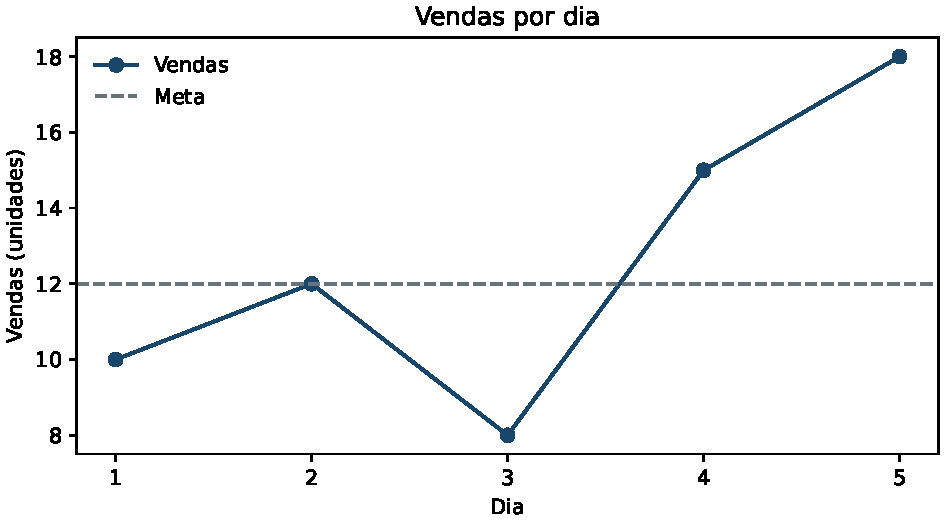
\includegraphics[width=0.76\linewidth]{figuras/linhas.pdf}

\raggedright
As vendas caem de \(12\) para \(8\) entre o segundo e o terceiro dia e voltam a subir até \(18\) no quinto. Os pontos mostram as contagens observadas em cada dia.
\end{minipage}

\needspace{33\baselineskip}
\subsection{Legendas para identificar as séries}
\label{sec:legendas}

Em um gráfico com várias séries, o argumento \codigo{label} dá um nome a cada série. A chamada a \codigo{ax.legend()} após o desenho das séries exibe esses nomes. A legenda usa esses nomes junto com a cor, o marcador e o estilo da linha de cada série \cite{matplotlib}.

\begin{exemplo}
import matplotlib.pyplot as plt

dias = [1, 2, 3, 4, 5]
loja_a = [10, 12, 8, 15, 18]
loja_b = [8, 9, 11, 13, 15]

fig, ax = plt.subplots(figsize=(6.3, 3.5), layout="constrained")
ax.plot(dias, loja_a, label="Loja A", marker="o", color="#19476B")
ax.plot(dias, loja_b, label="Loja B", marker="s",
        linestyle="--", color="#A45727")
ax.set(title="Vendas por loja", xlabel="Dia",
       ylabel="Vendas (unidades)", xticks=dias)
ax.legend(title="Loja", loc="upper left", frameon=False)
plt.show()
\end{exemplo}

\noindent\begin{minipage}{\linewidth}
\centering
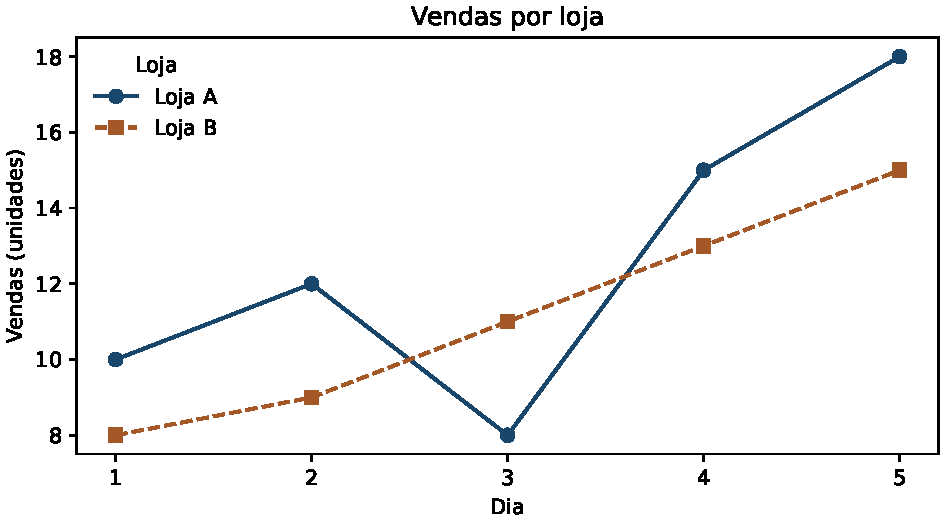
\includegraphics[width=0.76\linewidth]{figuras/legendas.pdf}

\raggedright
A linha contínua representa a Loja A e a tracejada representa a Loja B. No dia \(3\), a Loja B vendeu \(11\) unidades e a Loja A vendeu \(8\).
\end{minipage}

O argumento \codigo{title} dá um título à legenda. \codigo{loc="upper left"} posiciona a legenda no canto superior esquerdo. Se essa posição cobrir dados importantes, outra posição pode ser indicada. Com \codigo{loc="best"}, o Matplotlib escolhe entre as posições disponíveis.

\needspace{33\baselineskip}
\subsection{Gráfico de barras}

\codigo{ax.bar()} recebe as categorias e suas alturas. Neste exemplo, as alturas são as contagens de notas válidas por curso, obtidas com \codigo{value\_counts()}. A base zero permite comparar as alturas diretamente. Se \(c_i\) é o curso do registro \(i\) com nota válida, a altura da barra do curso \(c\) é
\[
  h_c=\sum_{i=1}^{n}\mathbf{1}(c_i=c).
\]
A função indicadora \(\mathbf{1}\) vale \(1\) quando a condição é verdadeira e \(0\) nos demais casos. A soma conta os registros que pertencem ao curso.

\begin{exemplo}
import matplotlib.pyplot as plt
from matplotlib.ticker import MaxNLocator

contagens = df_validas["curso"].value_counts().sort_index()

fig, ax = plt.subplots(figsize=(6.3, 3.5), layout="constrained")
barras = ax.bar(contagens.index, contagens.values, color="#19476B")
ax.set(title="Notas observadas por curso", xlabel="Curso",
       ylabel="Quantidade de notas", ylim=(0, 7))
ax.yaxis.set_major_locator(MaxNLocator(integer=True))
ax.bar_label(barras, padding=3)
plt.show()
\end{exemplo}

\noindent\begin{minipage}{\linewidth}
\centering
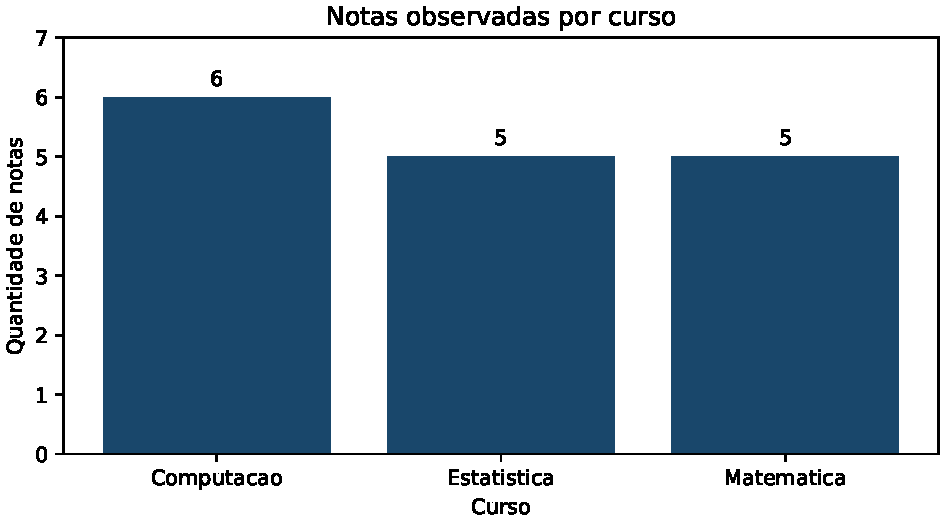
\includegraphics[width=0.76\linewidth]{figuras/barras.pdf}

\raggedright
Computação tem seis notas disponíveis. Estatística e Matemática têm cinco cada. Como a base original tem seis registros por curso, o gráfico ajuda a identificar onde há notas ausentes.
\end{minipage}

\needspace{33\baselineskip}
\subsection{Histograma}

O histograma resume uma variável numérica agrupando seus valores em intervalos. \codigo{ax.hist()} recebe as observações e usa \codigo{bins} para definir os intervalos. Um inteiro, como \codigo{bins=5}, pede cinco intervalos de mesma largura na faixa dos dados. Uma lista fornece os limites explicitamente. Com \codigo{[5, 6, 7, 8, 9, 10]}, os cinco intervalos têm largura \(1\).

Os intervalos incluem o limite esquerdo e excluem o direito. O último também inclui o limite direito. Assim, uma nota \(8{,}0\) entra no intervalo de \(8\) a \(9\), e uma nota \(10{,}0\) entraria no último \cite{matplotlib}.

Para notas \(x_1,\ldots,x_n\) e um intervalo \([b_j,b_{j+1})\), a altura em contagens é \(n_j\) e a frequência relativa é \(f_j\):
\[
  n_j=\sum_{i=1}^{n}\mathbf{1}(b_j\le x_i<b_{j+1}),
  \qquad f_j=\frac{n_j}{n}.
\]
No último intervalo, a desigualdade superior inclui o valor \(b_{j+1}\). No gráfico abaixo, o eixo vertical mostra \(n_j\).

\begin{exemplo}
import matplotlib.pyplot as plt
from matplotlib.ticker import MaxNLocator

notas = df_validas["nota"]
limites = [5, 6, 7, 8, 9, 10]

fig, ax = plt.subplots(figsize=(6.3, 3.5), layout="constrained")
alturas, _, _ = ax.hist(notas, bins=limites,
                       color="#19476B", edgecolor="white")
ax.set(title="Histograma das notas", xlabel="Nota",
       ylabel="Contagem", xticks=limites)
ax.yaxis.set_major_locator(MaxNLocator(integer=True))
print(alturas.astype(int).tolist())  # [2, 3, 4, 4, 3]
plt.show()
\end{exemplo}

\noindent\begin{minipage}{\linewidth}
\centering
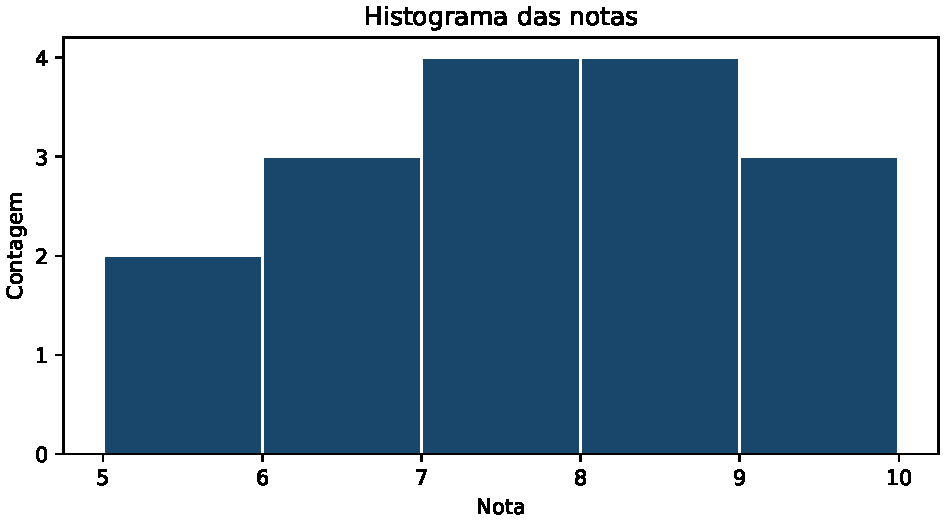
\includegraphics[width=0.76\linewidth]{figuras/distribuicao.pdf}

\raggedright
O gráfico tem quatro notas de \(7\) a menos de \(8\) e outras quatro de \(8\) a menos de \(9\). Cada intervalo contém \(4/16=25\%\) das notas observadas, e os dois juntos concentram \(50\%\).
\end{minipage}

A largura dos intervalos muda o que fica visível. Com poucos intervalos, detalhes podem ser agregados. Com muitos, uma base pequena pode produzir várias barras vazias. Ao comparar dois histogramas, usar os mesmos limites facilita a leitura. Valores fora desses limites ficam de fora do gráfico. Se \(n\) continua sendo o total original, as frequências \(n_j/n\) podem somar menos de \(100\%\).

\needspace{33\baselineskip}
\subsection{Boxplot}

\codigo{ax.boxplot()} resume a distribuição de uma variável. A caixa vai do primeiro ao terceiro quartil, e a linha dentro dela marca a mediana. Com a configuração padrão, os bigodes chegam até as observações mais extremas dentro dos limites de \(1{,}5\) vez o intervalo interquartil. Pontos além dos bigodes aparecem separadamente \cite{matplotlib}. Com \(Q_1\) e \(Q_3\) como limites da caixa, os limites para localizar os bigodes são
\[
  \mathrm{IQR}=Q_3-Q_1,\qquad
  L=Q_1-1{,}5\,\mathrm{IQR},\qquad U=Q_3+1{,}5\,\mathrm{IQR}.
\]
No exemplo, \(\mathrm{IQR}=8{,}50-6{,}625=1{,}875\). Os bigodes chegam às observações extremas dentro de \([L,U]\).

\begin{exemplo}
import matplotlib.pyplot as plt

notas = df_validas["nota"]

fig, ax = plt.subplots(figsize=(6.3, 3.4), layout="constrained")
ax.boxplot(notas, widths=0.4,
           medianprops={"color": "#19476B", "linewidth": 2})
ax.set(title="Boxplot das notas", ylabel="Nota", xticks=[])
plt.show()
\end{exemplo}

\noindent\begin{minipage}{\linewidth}
\centering
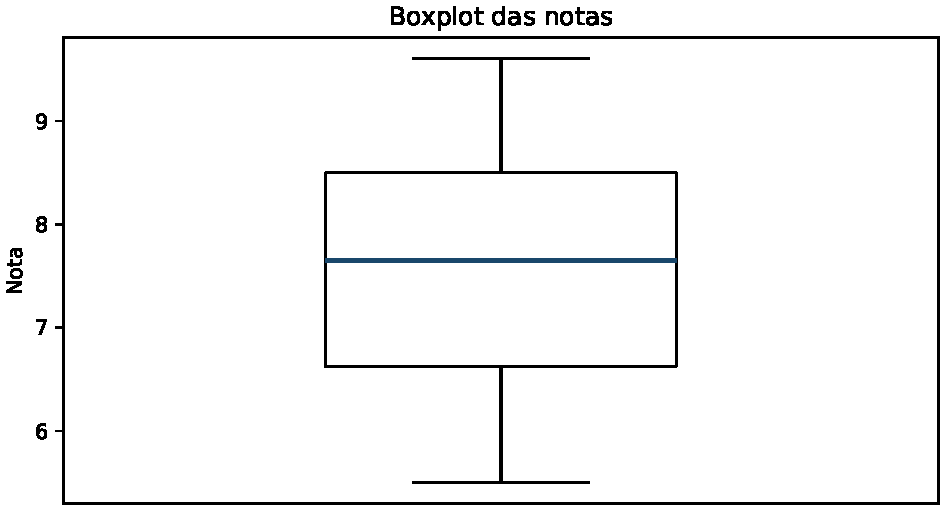
\includegraphics[width=0.76\linewidth]{figuras/boxplot.pdf}

\raggedright
A mediana é \(7{,}65\). A caixa delimita a metade central dos dados, entre \(6{,}625\) e \(8{,}50\). Neste caso, nenhuma observação fica além dos bigodes.
\end{minipage}

\needspace{33\baselineskip}
\subsection{Gráfico de dispersão}

\codigo{ax.scatter(x, y)} desenha um ponto para cada par de valores. No exemplo, cada ponto representa um participante. A coordenada horizontal indica horas de estudo e a vertical indica nota. O filtro de notas válidas é aplicado antes de selecionar as duas colunas para preservar o pareamento. O primeiro participante, por exemplo, aparece no ponto \((2,\;5{,}9)\). A correlação de Pearson resume a associação linear dos pares \((x_i,y_i)\):
\[
  r=\frac{\sum_i(x_i-\bar x)(y_i-\bar y)}
          {\sqrt{\sum_i(x_i-\bar x)^2}\,\sqrt{\sum_i(y_i-\bar y)^2}}.
\]
\(\bar x\) e \(\bar y\) são as médias das horas de estudo e das notas, respectivamente.

\begin{exemplo}
import matplotlib.pyplot as plt

fig_dispersao, ax = plt.subplots(figsize=(6.3, 3.6), layout="constrained")
ax.scatter(df_validas["horas_estudo"], df_validas["nota"],
           color="#19476B", alpha=0.85)
ax.set(title="Horas de estudo e nota",
       xlabel="Horas de estudo (h)", ylabel="Nota")
ax.set_axisbelow(True)
ax.grid(alpha=0.2)

r = df_validas["horas_estudo"].corr(df_validas["nota"])
print(round(r, 2))  # 0.96
plt.show()
\end{exemplo}

\noindent\begin{minipage}{\linewidth}
\centering
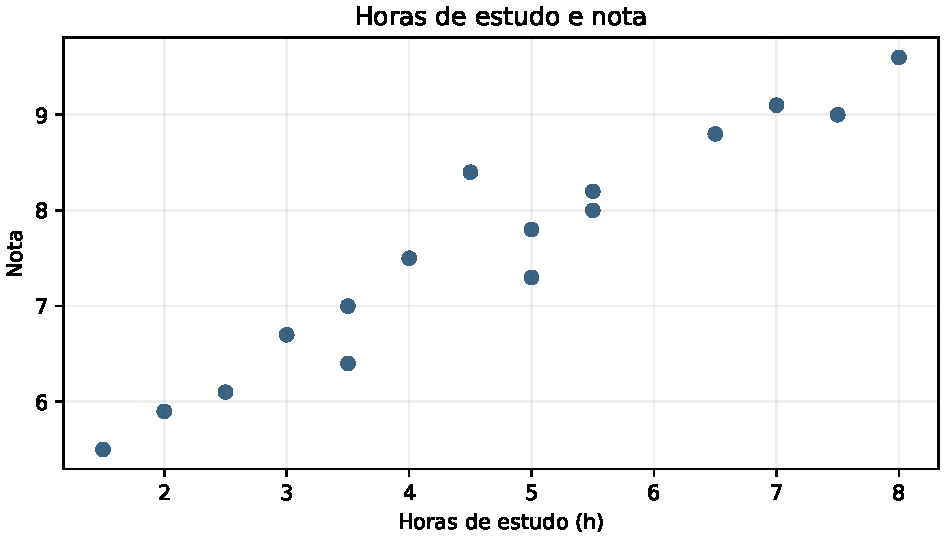
\includegraphics[width=0.62\linewidth]{figuras/dispersao.pdf}

\raggedright
A tendência ascendente e \(r=0{,}96\) indicam associação linear positiva na base simulada. Esse resultado, sozinho, é insuficiente para estabelecer causalidade.
\end{minipage}

\subsection{Salvar figuras}

\codigo{fig\_dispersao.savefig()} salva a figura de dispersão mesmo após a criação de outros gráficos. A extensão define o formato: PNG para imagem em pixels e PDF para preservar elementos vetoriais.

\begin{exemplo}
fig_dispersao.savefig("dispersao.png", dpi=200, bbox_inches="tight")
fig_dispersao.savefig("dispersao.pdf", bbox_inches="tight")
\end{exemplo}

Em scripts, a gravação pode preceder \codigo{plt.show()}. No Colab, os arquivos ficam no painel \textbf{Arquivos}.

\clearpage
\section{Exemplos de análise de dados}
\label{sec:analise}

Os dois exemplos usam a base de notas do guia. Primeiro contamos as notas ausentes. Depois comparamos as notas disponíveis por curso.

\subsection{Quantas notas estão faltando em cada curso?}

A contagem de notas ausentes usa \codigo{df}, a tabela original da Seção \ref{sec:ler}. Em um agrupamento, \codigo{size} conta todas as linhas e \codigo{count} conta os valores presentes na coluna. A diferença dá o número de notas ausentes. Dividir essa diferença pelo total do curso dá a proporção de registros sem nota.

\begin{exemplo}
cobertura = df.groupby("curso")["nota"].agg(
    total="size", com_nota="count"
)
cobertura["sem_nota"] = cobertura["total"] - cobertura["com_nota"]
cobertura["pct_sem_nota"] = (
    100 * cobertura["sem_nota"] / cobertura["total"]
).round(1)
print(cobertura)
\end{exemplo}

No gráfico empilhado, \codigo{bottom} faz a barra de notas ausentes começar no topo da barra de notas presentes. A altura total mostra o número de registros.

\begin{exemplo}
import matplotlib.pyplot as plt

fig, ax = plt.subplots(figsize=(6.3, 3.5), layout="constrained")
ax.bar(cobertura.index, cobertura["com_nota"],
       color="#19476B", label="Com nota")
ax.bar(cobertura.index, cobertura["sem_nota"],
       bottom=cobertura["com_nota"], color="#D69865",
       label="Sem nota")
ax.set(title="Registro de notas por curso", xlabel="Curso",
       ylabel="Quantidade de registros", ylim=(0, 8))
ax.legend(loc="upper center", ncol=2, frameon=False)
plt.show()
\end{exemplo}

\noindent\begin{minipage}{\linewidth}
\centering
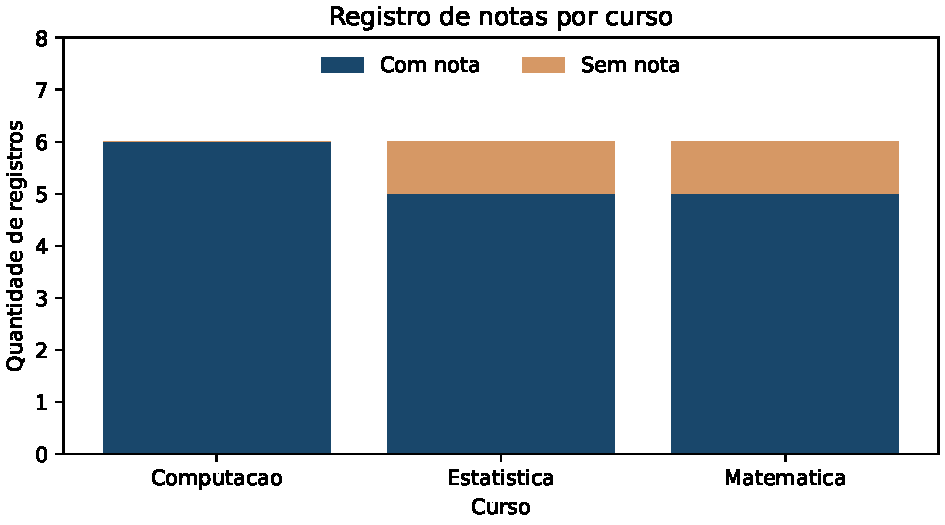
\includegraphics[width=0.66\linewidth]{figuras/notas-ausentes.pdf}

\raggedright
Estatística e Matemática têm uma nota ausente cada, ou \(16{,}7\%\) dos seus seis registros. Computação tem as seis notas. A causa das ausências depende de informações adicionais.
\end{minipage}

\needspace{34\baselineskip}
\subsection{Como as notas se distribuem por curso?}

A comparação usa as notas observadas em \codigo{df\_validas}, da Seção \ref{sec:ausentes}. \codigo{ax.boxplot()} recebe uma sequência de notas por curso. O eixo horizontal indica quantas observações entraram em cada grupo.

\begin{exemplo}
import matplotlib.pyplot as plt

notas_por_curso = []
rotulos = []
for curso, notas in df_validas.groupby("curso")["nota"]:
    notas_por_curso.append(notas.to_numpy())
    rotulos.append(f"{curso}\n(n={len(notas)})")

fig, ax = plt.subplots(figsize=(6.3, 3.6), layout="constrained")
ax.boxplot(notas_por_curso,
           medianprops={"color": "#19476B", "linewidth": 2})
ax.set_xticks(range(1, len(rotulos) + 1), rotulos)
ax.set(title="Notas por curso", ylabel="Nota")
plt.show()
\end{exemplo}

\noindent\begin{minipage}{\linewidth}
\centering
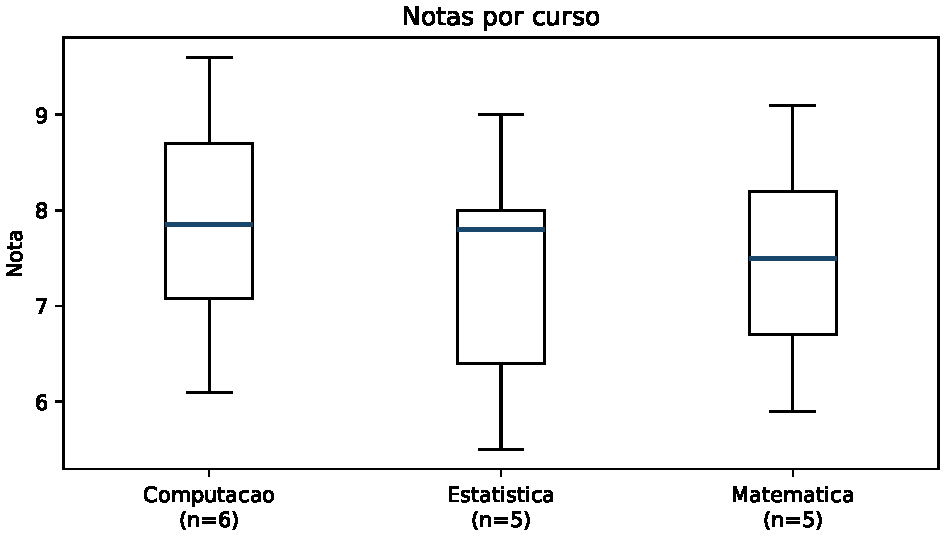
\includegraphics[width=0.69\linewidth]{figuras/notas-por-curso.pdf}

\raggedright
As medianas são \(7{,}85\), \(7{,}80\) e \(7{,}50\) em Computação, Estatística e Matemática, respectivamente. As caixas se sobrepõem e cada grupo tem apenas cinco ou seis notas. A comparação descreve esse conjunto simulado.
\end{minipage}

\needspace{6\baselineskip}
\subsection{Outras perguntas que viram gráficos}

\noindent\begin{tabularx}{\linewidth}{@{}>{\raggedright\arraybackslash}p{0.34\linewidth}>{\raggedright\arraybackslash}X>{\raggedright\arraybackslash}X@{}}
\toprule
\textbf{Pergunta} & \textbf{Como organizar os dados} & \textbf{Gráfico} \\
\midrule
Em que turno há mais atendimentos? & Contar atendimentos por turno. & Barras com uma categoria por turno. \\
Qual é o tempo de espera mais comum? & Reunir os tempos individuais, em minutos. & Histograma com intervalos de mesma largura. \\
Como o consumo de energia mudou durante o ano? & Somar o consumo de cada mês, em kWh. & Linhas com os meses na ordem do calendário. \\
O tempo de estudo e a nota variam juntos? & Usar os dois valores do mesmo participante e identificar seu curso. & Dispersão com um marcador por curso e legenda. \\
\bottomrule
\end{tabularx}\par

\clearpage
\section{Consulta rápida}
\setlength{\LTpre}{4pt}
\setlength{\LTpost}{6pt}

As tabelas agrupam os comandos pelo assunto. Cada linha traz um comando ou expressão e sua função no contexto dos exemplos do guia.

\needspace{9\baselineskip}
\subsection{Python}
\subsubsection*{Operadores}

\begin{longtable}{@{}>{\raggedright\arraybackslash}p{0.44\linewidth}@{\hspace{1em}}>{\raggedright\arraybackslash}p{\dimexpr0.56\linewidth-1em\relax}@{}}
\toprule
\textbf{Comando ou expressão} & \textbf{Uso} \\
\midrule
\endfirsthead
\toprule
\textbf{Comando ou expressão} & \textbf{Uso} \\
\midrule
\endhead
\midrule
\endfoot
\bottomrule
\endlastfoot
\codigo{x + y} & Somar valores numéricos. \\
\codigo{x - y} & Subtrair \(y\) de \(x\). \\
\codigo{x * y} & Multiplicar valores numéricos. \\
\codigo{x / y} & Dividir e obter um resultado de ponto flutuante. \\
\codigo{x // y} & Dividir e arredondar o quociente para baixo. \\
\codigo{x \% y} & Obter o resto da divisão. \\
\codigo{x ** y} & Elevar \(x\) à potência \(y\). \\
\codigo{x = valor} & Associar um valor ao nome \codigo{x}. \\
\codigo{x += y} & Atualizar um número somando \(y\) ao valor anterior. \\
\codigo{x == y} & Testar se os valores são iguais. \\
\codigo{x != y} & Testar se os valores são diferentes. \\
\codigo{x < y} & Testar se \(x\) é menor que \(y\). \\
\codigo{x <= y} & Testar se \(x\) é menor ou igual a \(y\). \\
\codigo{x > y} & Testar se \(x\) é maior que \(y\). \\
\codigo{x >= y} & Testar se \(x\) é maior ou igual a \(y\). \\
\codigo{a and b} & Exigir as duas condições booleanas. \\
\codigo{a or b} & Exigir pelo menos uma condição booleana. \\
\codigo{not a} & Inverter uma condição booleana. \\
\codigo{x in valores} & Testar se um valor pertence à coleção. \\
\codigo{x not in valores} & Testar se um valor está fora da coleção. \\
\codigo{x is None} & Identificar o valor usado para representar ausência. \\
\codigo{x is not None} & Testar se o valor é diferente de \codigo{None} por identidade. \\
\end{longtable}

\needspace{6\baselineskip}
\subsubsection*{Tipos e texto}

\begin{longtable}{@{}>{\raggedright\arraybackslash}p{0.44\linewidth}@{\hspace{1em}}>{\raggedright\arraybackslash}p{\dimexpr0.56\linewidth-1em\relax}@{}}
\toprule
\textbf{Comando ou expressão} & \textbf{Uso} \\
\midrule
\endfirsthead
\toprule
\textbf{Comando ou expressão} & \textbf{Uso} \\
\midrule
\endhead
\midrule
\endfoot
\bottomrule
\endlastfoot
\codigo{print(x)} & Exibir um valor na saída. \\
\codigo{type(x)} & Consultar o tipo de um objeto. \\
\codigo{int(x)} & Converter um valor para inteiro. \\
\codigo{float(x)} & Converter um valor para ponto flutuante. \\
\codigo{str(x)} & Converter um valor para texto. \\
\codigo{bool(x)} & Converter um valor para booleano. \\
\codigo{texto[i]} & Selecionar o caractere na posição \(i\). \\
\codigo{texto[inicio:fim]} & Extrair um trecho, excluindo o índice final. \\
\codigo{texto.strip()} & Remover espaços das extremidades. \\
\codigo{texto.lower()} & Retornar uma versão em letras minúsculas. \\
\codigo{texto.replace(a, b)} & Substituir cada ocorrência de \codigo{a} por \codigo{b}. \\
\codigo{texto.split(",")} & Separar o texto em partes usando a vírgula. \\
\codigo{" ".join(partes)} & Juntar textos separados por um espaço. \\
\codigo{f"\{nota:.2f\}"} & Apresentar a nota com duas casas decimais. \\
\codigo{f"\{proporcao:.0\%\}"} & Apresentar uma proporção como porcentagem inteira. \\
\end{longtable}

\needspace{6\baselineskip}
\subsubsection*{Coleções e repetição}

\begin{longtable}{@{}>{\raggedright\arraybackslash}p{0.44\linewidth}@{\hspace{1em}}>{\raggedright\arraybackslash}p{\dimexpr0.56\linewidth-1em\relax}@{}}
\toprule
\textbf{Comando ou expressão} & \textbf{Uso} \\
\midrule
\endfirsthead
\toprule
\textbf{Comando ou expressão} & \textbf{Uso} \\
\midrule
\endhead
\midrule
\endfoot
\bottomrule
\endlastfoot
\codigo{len(valores)} & Contar os itens de uma coleção. \\
\codigo{sum(valores)} & Somar os valores de uma coleção numérica. \\
\codigo{min(valores)} & Obter o menor valor. \\
\codigo{max(valores)} & Obter o maior valor. \\
\codigo{sorted(valores)} & Criar uma lista ordenada. \\
\codigo{lista.sort()} & Ordenar a lista existente. \\
\codigo{lista.append(x)} & Acrescentar um item ao final da lista. \\
\codigo{lista.extend(xs)} & Acrescentar os itens de outra coleção à lista. \\
\codigo{matriz[i][j]} & Ler a coluna \(j\) da linha \(i\) em uma lista de listas. \\
\codigo{(a, b)} & Criar uma tupla com dois elementos. \\
\codigo{set(valores)} & Criar um conjunto de valores distintos. \\
\codigo{dicionario.get(chave, padrao)} & Ler uma chave e retornar o padrão se ela estiver ausente. \\
\codigo{dicionario.items()} & Percorrer pares de chave e valor. \\
\codigo{range(inicio, fim, passo)} & Gerar inteiros até antes do limite final. \\
\codigo{enumerate(valores)} & Percorrer cada item junto com sua posição. \\
\codigo{zip(a, b)} & Agrupar elementos correspondentes até acabar a sequência mais curta. \\
\end{longtable}

\needspace{6\baselineskip}
\subsection{Estatística e probabilidade}

\begin{longtable}{@{}>{\raggedright\arraybackslash}p{0.44\linewidth}@{\hspace{1em}}>{\raggedright\arraybackslash}p{\dimexpr0.56\linewidth-1em\relax}@{}}
\toprule
\textbf{Comando ou expressão} & \textbf{Uso} \\
\midrule
\endfirsthead
\toprule
\textbf{Comando ou expressão} & \textbf{Uso} \\
\midrule
\endhead
\midrule
\endfoot
\bottomrule
\endlastfoot
\codigo{np.unique(x, return\_counts=True)} & Obter valores distintos e suas contagens. \\
\codigo{rotulos[contagens == maior]} & Identificar as modas quando \codigo{maior} é a maior contagem. \\
\codigo{np.count\_nonzero(mascara)} & Contar as posições verdadeiras de uma máscara. \\
\codigo{round(x, 2)} & Arredondar um número para duas casas decimais. \\
\codigo{binom.pmf(k, n, p)} & Calcular a probabilidade de exatamente \(k\) sucessos em \(n\) tentativas binomiais. \\
\codigo{poisson.pmf(k, mu)} & Calcular a probabilidade de exatamente \(k\) ocorrências para a média informada. \\
\end{longtable}

\needspace{9\baselineskip}
\subsection{NumPy}
\subsubsection*{Criação, formato e seleção}

\begin{longtable}{@{}>{\raggedright\arraybackslash}p{0.44\linewidth}@{\hspace{1em}}>{\raggedright\arraybackslash}p{\dimexpr0.56\linewidth-1em\relax}@{}}
\toprule
\textbf{Comando ou expressão} & \textbf{Uso} \\
\midrule
\endfirsthead
\toprule
\textbf{Comando ou expressão} & \textbf{Uso} \\
\midrule
\endhead
\midrule
\endfoot
\bottomrule
\endlastfoot
\codigo{np.array(lista)} & Criar um array a partir de uma sequência. \\
\codigo{np.zeros((l, c))} & Criar uma matriz de zeros com \(l\) linhas e \(c\) colunas. \\
\codigo{np.ones(n)} & Criar um vetor de uns com \(n\) elementos. \\
\codigo{np.arange(a, b, p)} & Gerar valores com passo \(p\), excluindo \(b\) para passos inteiros. \\
\codigo{np.linspace(a, b, n)} & Gerar \(n\) pontos igualmente espaçados. \\
\codigo{arr.shape} & Consultar o tamanho de cada dimensão. \\
\codigo{arr.ndim} & Consultar o número de dimensões. \\
\codigo{arr.dtype} & Consultar o tipo dos elementos. \\
\codigo{arr.reshape(l, c)} & Reorganizar o array com \(l\) linhas e \(c\) colunas. \\
\codigo{arr[i, j]} & Ler a entrada da linha \(i\) e coluna \(j\). \\
\codigo{arr[:, 1]} & Selecionar a segunda coluna. \\
\codigo{arr[arr >= 7]} & Selecionar elementos de acordo com uma máscara booleana. \\
\codigo{a.T} & Obter a matriz transposta. \\
\codigo{a * b} & Multiplicar elementos em posições correspondentes de arrays compatíveis. \\
\codigo{a @ b} & Calcular o produto matricial. \\
\end{longtable}

\needspace{6\baselineskip}
\subsubsection*{Operações e estatísticas}

\begin{longtable}{@{}>{\raggedright\arraybackslash}p{0.44\linewidth}@{\hspace{1em}}>{\raggedright\arraybackslash}p{\dimexpr0.56\linewidth-1em\relax}@{}}
\toprule
\textbf{Comando ou expressão} & \textbf{Uso} \\
\midrule
\endfirsthead
\toprule
\textbf{Comando ou expressão} & \textbf{Uso} \\
\midrule
\endhead
\midrule
\endfoot
\bottomrule
\endlastfoot
\codigo{arr.sum(axis=0)} & Somar os valores de cada coluna. \\
\codigo{arr.sum(axis=1)} & Somar os valores de cada linha. \\
\codigo{np.min(arr)} & Obter o menor elemento. \\
\codigo{np.max(arr)} & Obter o maior elemento. \\
\codigo{np.mean(arr)} & Calcular a média. \\
\codigo{np.nanmean(arr)} & Calcular a média desconsiderando \codigo{NaN}. \\
\codigo{np.median(arr)} & Calcular a mediana. \\
\codigo{np.var(arr, ddof=1)} & Calcular a variância amostral com divisor \(n-1\). \\
\codigo{np.std(arr, ddof=1)} & Calcular o desvio padrão amostral com divisor \(n-1\). \\
\codigo{np.percentile(arr, q)} & Calcular o percentil \(q\). \\
\codigo{np.corrcoef(x, y)} & Calcular a matriz de correlação de Pearson. \\
\end{longtable}

\needspace{9\baselineskip}
\subsection{pandas}
\subsubsection*{Leitura e inspeção}

\begin{longtable}{@{}>{\raggedright\arraybackslash}p{0.44\linewidth}@{\hspace{1em}}>{\raggedright\arraybackslash}p{\dimexpr0.56\linewidth-1em\relax}@{}}
\toprule
\textbf{Comando ou expressão} & \textbf{Uso} \\
\midrule
\endfirsthead
\toprule
\textbf{Comando ou expressão} & \textbf{Uso} \\
\midrule
\endhead
\midrule
\endfoot
\bottomrule
\endlastfoot
\codigo{pd.read\_csv(caminho)} & Ler um arquivo CSV. \\
\codigo{pd.Series(valores)} & Criar uma série com valores e índice. \\
\codigo{pd.DataFrame(registros)} & Criar uma tabela a partir de registros. \\
\codigo{df.head(3)} & Exibir as três primeiras linhas. \\
\codigo{df.tail(2)} & Exibir as duas últimas linhas. \\
\codigo{df.info()} & Exibir tipos e contagens de valores presentes por coluna. \\
\codigo{df.shape} & Consultar número de linhas e colunas. \\
\codigo{df.columns} & Consultar os nomes das colunas. \\
\codigo{df.describe()} & Gerar um resumo estatístico das colunas numéricas. \\
\end{longtable}

\needspace{6\baselineskip}
\subsubsection*{Seleção, limpeza e transformação}

\begin{longtable}{@{}>{\raggedright\arraybackslash}p{0.44\linewidth}@{\hspace{1em}}>{\raggedright\arraybackslash}p{\dimexpr0.56\linewidth-1em\relax}@{}}
\toprule
\textbf{Comando ou expressão} & \textbf{Uso} \\
\midrule
\endfirsthead
\toprule
\textbf{Comando ou expressão} & \textbf{Uso} \\
\midrule
\endhead
\midrule
\endfoot
\bottomrule
\endlastfoot
\codigo{df["nota"]} & Selecionar uma coluna como série. \\
\codigo{df[["curso", "nota"]]} & Selecionar duas colunas como tabela. \\
\codigo{df.iloc[:3]} & Selecionar as três primeiras linhas pela posição. \\
\codigo{df.loc[0, "nota"]} & Selecionar a célula pelo rótulo da linha e da coluna. \\
\codigo{df.loc[mascara]} & Selecionar as linhas marcadas como verdadeiras. \\
\codigo{serie.isin(valores)} & Criar uma máscara de pertencimento. \\
\codigo{df.sort\_values("nota")} & Ordenar as linhas pela nota. \\
\codigo{df.isna()} & Identificar células com valores ausentes. \\
\codigo{mascara.sum()} & Contar valores verdadeiros por coluna de uma máscara booleana. \\
\codigo{df.dropna(subset=["nota"])} & Remover linhas com nota ausente. \\
\codigo{serie.fillna(valor)} & Preencher valores ausentes de uma série. \\
\codigo{pd.to\_numeric(serie, errors="coerce")} & Converter valores e sinalizar entradas inválidas como ausentes. \\
\codigo{serie.apply(funcao)} & Aplicar uma função a cada valor da série. \\
\codigo{df.copy()} & Criar uma cópia da tabela para análise separada. \\
\end{longtable}

\needspace{6\baselineskip}
\subsubsection*{Resumo, junção e exportação}

\begin{longtable}{@{}>{\raggedright\arraybackslash}p{0.44\linewidth}@{\hspace{1em}}>{\raggedright\arraybackslash}p{\dimexpr0.56\linewidth-1em\relax}@{}}
\toprule
\textbf{Comando ou expressão} & \textbf{Uso} \\
\midrule
\endfirsthead
\toprule
\textbf{Comando ou expressão} & \textbf{Uso} \\
\midrule
\endhead
\midrule
\endfoot
\bottomrule
\endlastfoot
\codigo{serie.value\_counts()} & Contar ocorrências de cada valor. \\
\codigo{df.groupby("curso")} & Agrupar as linhas de acordo com o curso. \\
\codigo{grupo.agg(medidas)} & Calcular as medidas indicadas para cada grupo. \\
\codigo{grupo.count()} & Contar valores presentes por grupo. \\
\codigo{grupo.size()} & Contar todas as linhas por grupo. \\
\codigo{serie.quantile(0.5)} & Calcular o quantil de ordem \(0{,}5\), a mediana. \\
\codigo{serie.corr(outra)} & Calcular a correlação de Pearson entre duas séries alinhadas pelo índice. \\
\codigo{df.merge(outro, on="id")} & Combinar tabelas pela chave \codigo{id}. \\
\codigo{df.reset\_index()} & Levar o índice antigo para uma coluna e criar um índice numérico. \\
\codigo{df.to\_csv("saida.csv", index=False)} & Exportar a tabela para CSV sem gravar o índice. \\
\end{longtable}

\needspace{9\baselineskip}
\subsection{Matplotlib}
\subsubsection*{Criação e leitura dos gráficos}

\begin{longtable}{@{}>{\raggedright\arraybackslash}p{0.44\linewidth}@{\hspace{1em}}>{\raggedright\arraybackslash}p{\dimexpr0.56\linewidth-1em\relax}@{}}
\toprule
\textbf{Comando ou expressão} & \textbf{Uso} \\
\midrule
\endfirsthead
\toprule
\textbf{Comando ou expressão} & \textbf{Uso} \\
\midrule
\endhead
\midrule
\endfoot
\bottomrule
\endlastfoot
\codigo{plt.subplots()} & Criar a figura e os eixos. \\
\codigo{ax.plot(x, y)} & Conectar os pontos na ordem fornecida. \\
\codigo{ax.axhline(y)} & Inserir uma linha horizontal de referência. \\
\codigo{ax.bar(categorias, alturas)} & Comparar valores por categoria. \\
\codigo{ax.bar\_label(barras)} & Exibir os valores junto às barras. \\
\codigo{ax.hist(valores, bins=limites)} & Contar observações em intervalos. \\
\codigo{ax.boxplot(valores)} & Resumir a distribuição com mediana, quartis e bigodes. \\
\codigo{ax.scatter(x, y)} & Mostrar a relação entre duas variáveis numéricas. \\
\codigo{ax.set(title=..., xlabel=..., ylabel=...)} & Definir título e rótulos dos eixos. \\
\codigo{ax.set\_xticks(posicoes, rotulos)} & Definir as posições e os rótulos no eixo horizontal. \\
\codigo{ax.grid(alpha=0.2)} & Exibir linhas de grade com transparência. \\
\codigo{label="Série"} & Nomear um elemento quando ele é desenhado. \\
\codigo{ax.legend(loc="upper left")} & Exibir a legenda no canto superior esquerdo. \\
\codigo{plt.show()} & Exibir a figura. \\
\codigo{fig.savefig("grafico.png", dpi=200)} & Salvar a figura em um arquivo. \\
\end{longtable}

\subsection{Onde continuar}

A documentação do Python em português reúne tutoriais e a referência da linguagem \cite{python}. As documentações de NumPy, pandas, Matplotlib e SciPy descrevem parâmetros e apresentam exemplos de uso \cite{numpy,pandas,matplotlib,scipy}. A documentação do Jupyter aborda a execução e a organização de notebooks \cite{jupyter}.

\clearpage
\section*{Uso de inteligência artificial}
O ChatGPT (Codex), da OpenAI, foi usado como apoio na revisão do texto, na organização em LaTeX e na preparação e verificação dos exemplos de código \cite{openai-codex}.

\printbibliography[heading=bibintoc,title={Referências}]

\end{document}
